\documentclass{article}
\usepackage[left=3.5cm,top=2.5cm,right=3.5cm,bottom=2.5cm]{geometry}
\usepackage[utf8]{inputenc}
\usepackage[spanish]{babel}
\usepackage{listings}
\usepackage{graphicx}
\graphicspath{ {images/} }
\usepackage{cite}



\usepackage[T1]{fontenc}

\usepackage{times}

\usepackage{color}
\definecolor{gray97}{gray}{.97}
\definecolor{gray75}{gray}{.75}
\definecolor{gray45}{gray}{.45}


\lstset{ frame=Ltb,
framerule=0pt,
aboveskip=0.5cm,
framextopmargin=3pt,
framexbottommargin=3pt,
framexleftmargin=0.5cm,%0.4cm
framesep=0pt,
rulesep=.4pt,
backgroundcolor=\color{gray97},
rulesepcolor=\color{black},
%
stringstyle=\ttfamily,
showstringspaces = false,
basicstyle=\small\ttfamily,
commentstyle=\color{gray45},
keywordstyle=\bfseries,
%
numbers=left,
numbersep=15pt,
numberstyle=\tiny,
numberfirstline = false,
breaklines=true,
}

% minimizar fragmentado de listados
\lstnewenvironment{listing}[1][]
{\lstset{#1}\pagebreak[0]}{\pagebreak[0]}

\lstdefinestyle{consola}
{basicstyle=\scriptsize\bf\ttfamily,
backgroundcolor=\color{gray75},
}

\lstdefinestyle{C++}
{language=C++}


\begin{document}


\begin{titlepage}
    \begin{center}
        \vspace*{1cm}
            
        \Huge
        \textbf{Desafío 1: Nada es lo que parece}
            
        \vspace{0.5cm}
        \LARGE
        Informa 2 S.A.S.
            
        \vspace{1.5cm}
            
        \textbf{Víctor Manuel Jiménez García\\
                José Miguel Jaramillo Sánchez\\
                Sebastián García Morales}

        \vfill
            
        \vspace{0.8cm}
            
        \Large
        Departamento de Ingeniería Electrónica y Telecomunicaciones\\
        Universidad de Antioquia\\
        Medellín\\
        Febrero 17 de 2022
    \end{center}
\end{titlepage}

\tableofcontents

\newpage
\section{Objetivos}\label{objetivos}
\begin{itemize}
    \item Aplicar los conocimientos adquiridos a lo largo del curso, demostrando apropiación de los fundamentos básicos del lenguaje de programación C++.
    \item Desarrollar habilidades de investigación y redacción que permitan la adquisición de nuevos conocimientos con el fin de solucionar problemas de la vida real.
    \item Demostrar la importancia y utilidad de la programación por hardware, así como el uso de módulos físicos para optimizar el uso de software en un diseño.
    \item Diseñar un aplicativo en la plataforma de Arduino integrando programación de C++ para solucionar un desafío  propuesto.
\end{itemize}
\section{Introducción}\label{intro}
La solución de problemas es por lejos, una de las habilidades mas importantes para el ser humano, le ha permitido afrontar dificultades y superar los obstáculos que se le han presentado a lo largo de toda su existencia. La capacidad de adaptarse a su entorno, aprender de él y aprovechar sus recursos son una manifestación natural del desarrollo de esta habilidad.\\
La ingeniería en sí misma se modela bajo esta premisa primitiva, que hoy en día se vale de un largo historial de descubrimientos, ciencias y conocimientos en pro de solucionar aquellos problemas que aun quedan sin resolver y preparándose para aquellos que están por venir.\\

Este proyecto presenta aquellos rasgos fundamentales de la solución de problemas por medio de la solución del desafio propuesto, cuyo eje central consiste en la implementación de un sistema de encriptación que permite cifrar los datos de un sistema a otro, usando una estrategia de programación híbrida entre software y hardware, y que permita desencriptar exitosamente los datos en el receptor de acuerdo a una serie de reglas descritas mas adelante en este mismo documento.\\

La primera parte de este trabajo contiene todos aquellos conceptos previos necesarios para poder plantear la solución correcta, la definicion de los dispositivos que usaremos para transmitir y recibir información, las características de la comunicación serial y la utilidad del integrado 74HC595, un registro de desplazamientos que nos permitirá extraer los datos de la trama serial y paralelizarla para alimentar un sistema de comparación a base de lógica combinacional con el fin de tomar decisiones.\\

La segunda parte expone paso a paso la ejecución de la solución por medio de una implementación modular, una forma de abordar el problema como una colección de otros mas pequeños, volviendo mas eficiente y efectiva la aplicación de la solución, pues el trabajo se vuelve delegable y hay un mejor enfoque para cada seccion del sistema. Durante toda el desarrollo de la solucion haremos uso de herramientas que faciliten nuestro trabajo como lo es TinkerCAD, un simulador online que permite realizar montajes electronicos y programar dispositivos Arduino; QT Creator una plataforma de desarrollo basado en lenguaje C++ cuyo depurador facilita el encontrar errores y probar nuestros codigos; Git y GitHUB, herramientas de control de versiones y respositorio que posibilitan el trabajo colaborativo.

\vspace{3cm}

\section{Marco Teórico}\label{marco}

\subsection{Conocimientos previos}

A la hora de enfrentarse a un desafío lo más recomendable es dividirlo en varias etapas para trabajarlo más fácilmente, una primera etapa sería realizar una investigación de conceptos y componentes propuestos en el desafío. En este caso es necesario investigar el concepto de transferir información de forma serial y paralela cómo también identificar características, funcionalidades, arquitectura, conexiones, alcances y limitaciones del circuito integrado 75HC595, por otro lado, ¿qué es un Arduino? Y ¿cómo unirlo al circuito integrado mencionado anteriormente para lograr solucionar el desafío completo?\\

Arduino es una plataforma de desarrollo basada en una placa electrónica de hardware libre que incorpora un microcontrolador reprogramable  y una serie de pines hembra. Estos permiten establecer conexiones entre el microcontrolador y los diferentes sensores y actuadores de una manera muy sencilla (principalmente con cables DuPont).\cite{arduinowebsite}\\

Este dispositivo es el que nos permitirá recibir los datos ingresados por el usuario y realizar la conversión a binario, además de funcionar tanto de transmisor como de receptor en el sistema de encriptación.\\

La comunicación entre Arduinos se realizará de forma serial, que es el proceso de enviar datos de carácter binario un bit a la vez, esto provee la ventaja de mantener la interfaz transmisor - receptor de forma simple y eficiente.\cite{serialsite}\\
Por lo tanto, para desencriptar, es necesario paralelizar dicha secuencia de bits que luego serán las entradas de un circuito de lógica combinacional encargado de comparar los datos de acuerdo a los parámetros de desencriptación.

Paralelizar no es más que llevar la secuencia de bits que se desplazan como una sola fila, y transformarla en una columna. De esta forma si se tiene una secuencia serial de n bits, al paralelizar, el resultado es una columna de bits de n filas.

\begin{figure}[!ht]
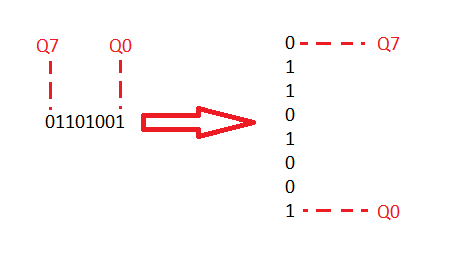
\includegraphics[width=8cm]{paralelizacion.png}
\centering
\caption{Ejemplo de paralelización}
\end{figure}

Esta acción de paralelizar la llevará a cabo el circuito integrado 74HC595 también conocido como Registro de desplazamiento. Este chip de 16 pines, recibe una secuencia de 8 bits en un solo pin, y los va almacenando en cada una de las salidas para luego ser liberados como 8 señales independientes.\\

Dos definiciones que se deben de tener en cuenta para entender mejor el funcionamiento de todo el sistema son: comunicación síncrona y comunicación asíncrona.\\

\noindent\textbf{Comunicación sincrónica:} Se da cuando el intercambio de mensajes sucede en tiempo real. Requiere que las dos partes (emisor y receptor) estén presentes en el mismo tiempo y espacio, ya sea físico o virtual. Por ejemplo, las llamadas telefónicas, las reuniones en la oficina o las videoconferencias.\\

\noindent\textbf{Comunicación asíncrona:} Sucede cuando los mensajes se intercambian sin importar el tiempo. Es decir, que no necesitan la atención inmediata del receptor, quien puede responder en el momento que decida o pueda hacerlo. Estamos hablando de medios como el correo electrónico, foros en línea, chats, mensajes de texto y documentos colaborativos.\cite{sincrosite}\\

En este caso, la comunicación se da de forma síncrona con ayuda de un pulso de reloj.
En electrónica y especialmente en circuitos digitales síncronos, una señal de reloj es una señal usada para coordinar las acciones de dos o más circuitos, esta señal oscila entre estado alto y bajo, también conocido como flanco de subida y de bajada, respectivamente, y gráficamente toma la forma de una onda cuadrada.\cite{relojsite}\\

\begin{figure}[!ht]
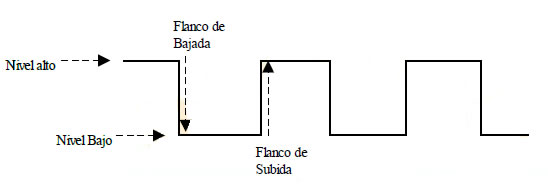
\includegraphics[width=8cm]{flanco1.jpg}
\centering
\caption{Diagrama de tiempo de una señal de reloj}
\end{figure}

A continuación se muestra la distribución de pines del circuito integrado 74HC595\\

\begin{figure}[!ht]
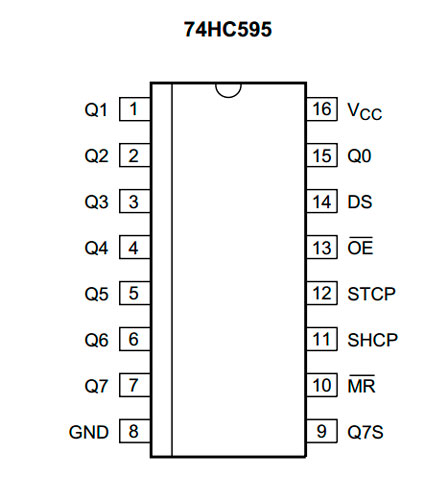
\includegraphics[width=5cm]{74HC595.jpg}
\centering
\caption{Pines IC 74HC595}
\end{figure}

\noindent\textbf{Entradas:}\\
\indent \textbf{GND} (pin 8): conexión a tierra (0 V)\\
\indent \textbf{GND} (pin 10): reinicio del registro (activo bajo)\\
\indent \textbf{SHCP} (pin 11): señal de reloj \\
\indent \textbf{STCP} (pin 12): pulso para liberar los datos \\
\indent \textbf{GND} (pin 13): habilitar salida del registro (activo bajo)\\
\indent \textbf{DS} (pin 14): entrada de datos serial \\
\indent \textbf{VCC} (pin 16): conexión a fuente de voltaje (5 V)\\

\noindent\textbf{Salidas:}\\ 
\indent \textbf{Q0-Q7} (pines 1-7 y 15 ): salida de datos\\
\indent \textbf{Q7S} (pin 9): salida de datos serial\\
\vspace{1cm}

El funcionamiento es el siguiente, la información serial entra por el \textbf{DS (pin 14)}, el integrado recibe cada bit cuando ocurre un flanco de subida por el \textbf{SHCP (pin 11)} y lo almacena en la salida de más bajo valor \textbf{Q0 (pin 15)}, a medida que van entrando más bits, los datos que se habían almacenado anteriormente se van desplazando desde \textbf{Q0} hasta \textbf{Q7} hasta completar el byte. Una vez hecho esto, se manda un flanco de subida en \textbf{STCP (pin 12)}, que se encarga de liberar los datos almacenados.\\

\noindent De esta forma el primer bit que entra, queda en la salida \textbf{Q7} y el último en la salida \textbf{Q0}.
Para ingresar un nuevo byte se debe borrar la información del registro, esto se hace mandando un flanco de bajada al pin \textbf{MR (pin 10)} y luego activando la salida del registro \textbf{(pin 12)}.\cite{74hc595datasheet}

\section{Análisis del problema} \label{analisis}

\subsection{Panorama del problema}


El problema consiste en transferir una secuencia de bits encriptados desde un Arduino a otro de forma serial, desencriptándola antes de que llegue al receptor usando lógica combinacional y un registro de desplazamiento.\\

\begin{figure}[!ht]
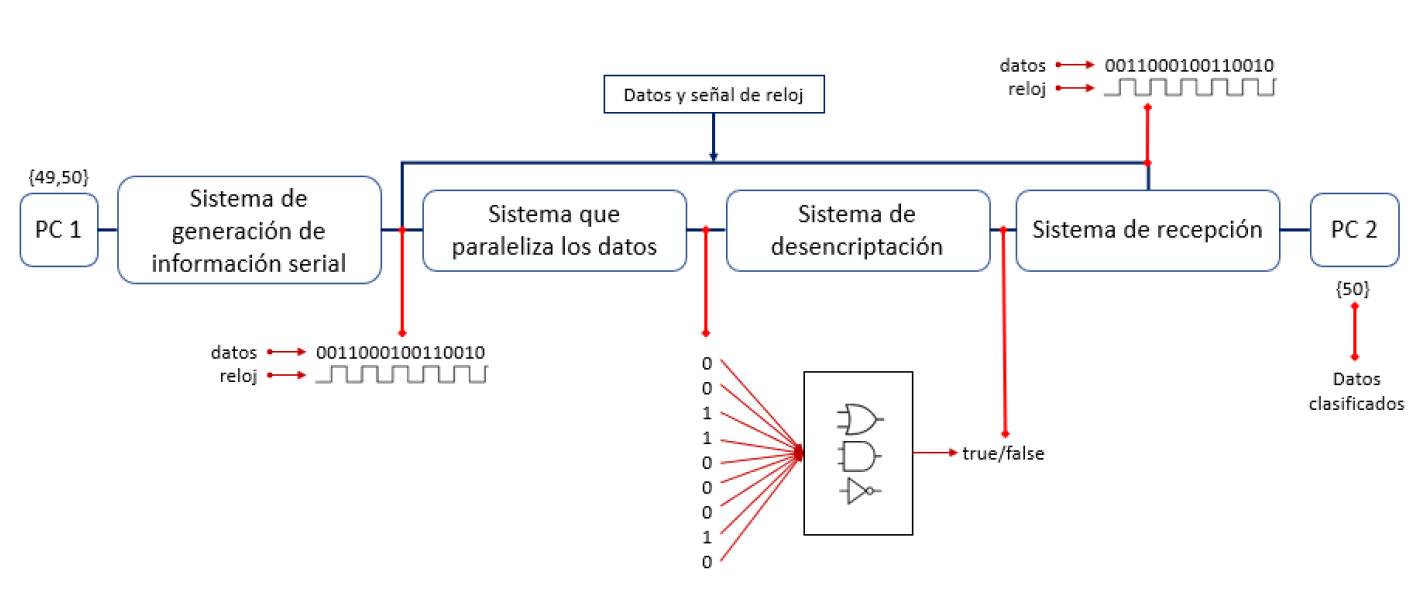
\includegraphics[width=10cm]{esquema.PNG}
\centering
\caption{Esquema del sistema a implementar. Recuperado de \cite{augusto}}
\end{figure}

Inicialmente, la información se dará al Arduino en forma de arreglo numérico ingresándola en el código del microcontrolador, este se encargará de realizar la conversión a binario y de generar los pulsos de reloj y reset necesarios para usar en el circuito integrado 74HC595.\\

La salida serial del Arduino, así como las señales de sincronización entraran al 74HC595 que se encargará de paralelizar los datos, entregando 8 salidas diferentes, que a su vez alimentaran las compuertas de un circuito de lógica combinacional con una única salida True o False de acuerdo a una referencia dada. En nuestro caso esta referencia es el numero 127\\

Al Arduino receptor le entrarán el reloj y los datos en forma serial; sin embargo, solo admitirá aquella información que bajo ciertas condiciones dé como resultado un True en la lógica combinacional, en otras palabras, la lógica combinacional funcionará como un comparador que le dirá al receptor que información es correcta y cuál deberá ser descartada, realizando de esta forma la desencriptación de los datos.\\

Cuando el arreglo tenga el numero 127, que es nuestra referencia, los datos validos serán el promedio con redondeo de los 3 datos siguientes\\
\begin{figure}[!ht]
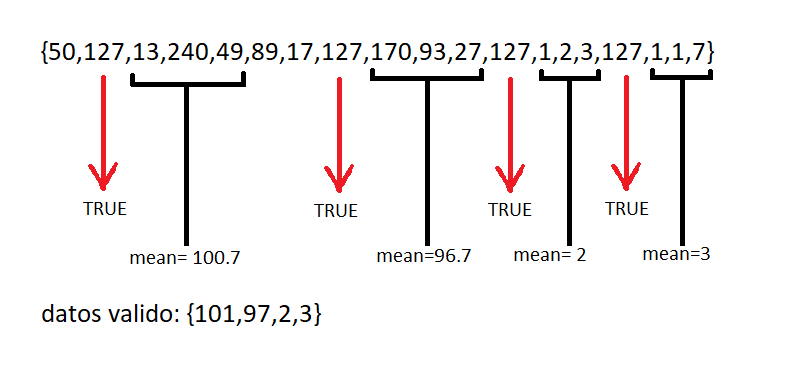
\includegraphics[width=10cm]{reglas.png}
\centering
\caption{Ejemplo de aplicacion de la regla de desencriptacion}
\end{figure}
En la siguiente sección se presentarán a detalle todas las etapas de solución.
\vspace{2cm}
\subsection{Etapas de la solución}

Para afrontar el problema, se opta por dividirlo en distintas etapas o módulos, de forma que se pueda verificar el correcto funcionamiento de cada uno por separado. Una vez hecho esto se juntan todas las etapas para posteriormente construir el modelo final del sistema.\\
\subsubsection{Circuito con el integrado 74HC595}

Como primera etapa se revisa el funcionamiento del circuito integrado 74HC595 en el simulador Tinkercad con ayuda de LEDS, botones y conmutadores. 

Para la alimentación se usa una fuente de voltaje de 5 V, se realizan las respectivas conexiones de forma que cada LED represente una salida del integrado y por facilidad se realiza el montaje solo para 4 bits. Las funciones de reloj, datos, y liberación de datos se realizan con conmutadores y botones.\\

Para ingresar un dato se usa el botón reloj, que permitirá la entrada de un 1 o un 0, de acuerdo a la posición que tenga los conmutadores deslizantes (la izquierda representa 1 y la derecha 0). Luego de tener 4 datos ingresados se presiona el botón reloj de registro, mostrando los datos ingresados en los leds.\\

Una vez montado el circuito, se evidencia que, aunque su comportamiento es el esperado, no se permitía ingresar más información nueva ni borrar la existente, esto se debía a que no se había agregado un botón de reset en el pin 10 del integrado. Esta corrección ya se muestra en el circuito de la Figura 6.\\

\begin{figure}[ht]
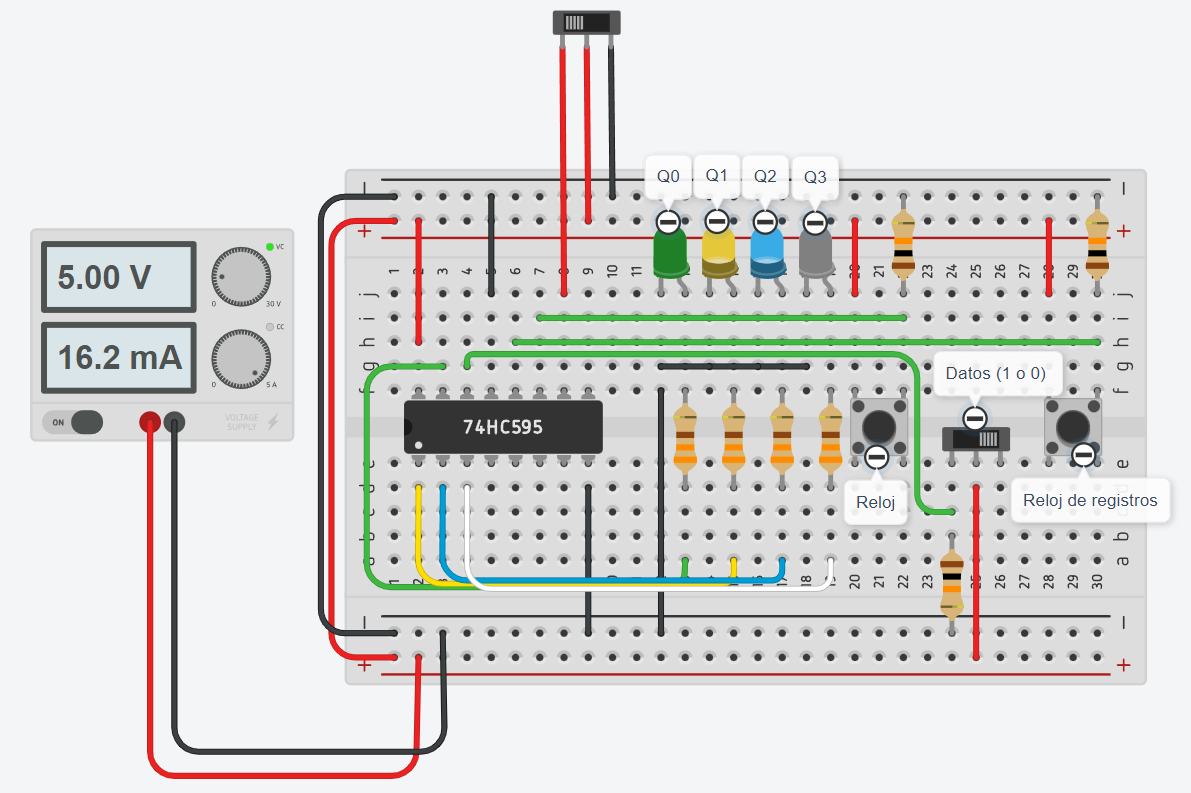
\includegraphics[width=7cm]{montaje0.PNG}
\centering
\caption{Primer montaje con el 74HC595}
\end{figure}
\vspace{2cm}
Después de haber garantizado el funcionamiento con botones y conmutadores, se procede a reemplazarlos por las salidas digitales del Arduino, en este caso el reset, el reloj de registro, la entrada de datos y el reloj están conectados a los pines 4, 5, 6 y 7 respectivamente. También se usan LEDS adicionales para llevar control de los pulsos que salen del Arduino como puede verse en la Figura 7.

El pulso de reloj principal es implementado internamente en el Arduino con ayuda de un ciclo y delays. Los datos a transmitir provienen de un arreglo de unos y ceros que es recorrido con un for y cuyo valor solo es liberado  cuando ocurre un flanco de subida del reloj. El reloj de registros tendrá un periodo de 4 veces el periodo del reloj principal, pues para este caso se está trabajando solo con 4 bits.

\begin{figure}[!ht] 
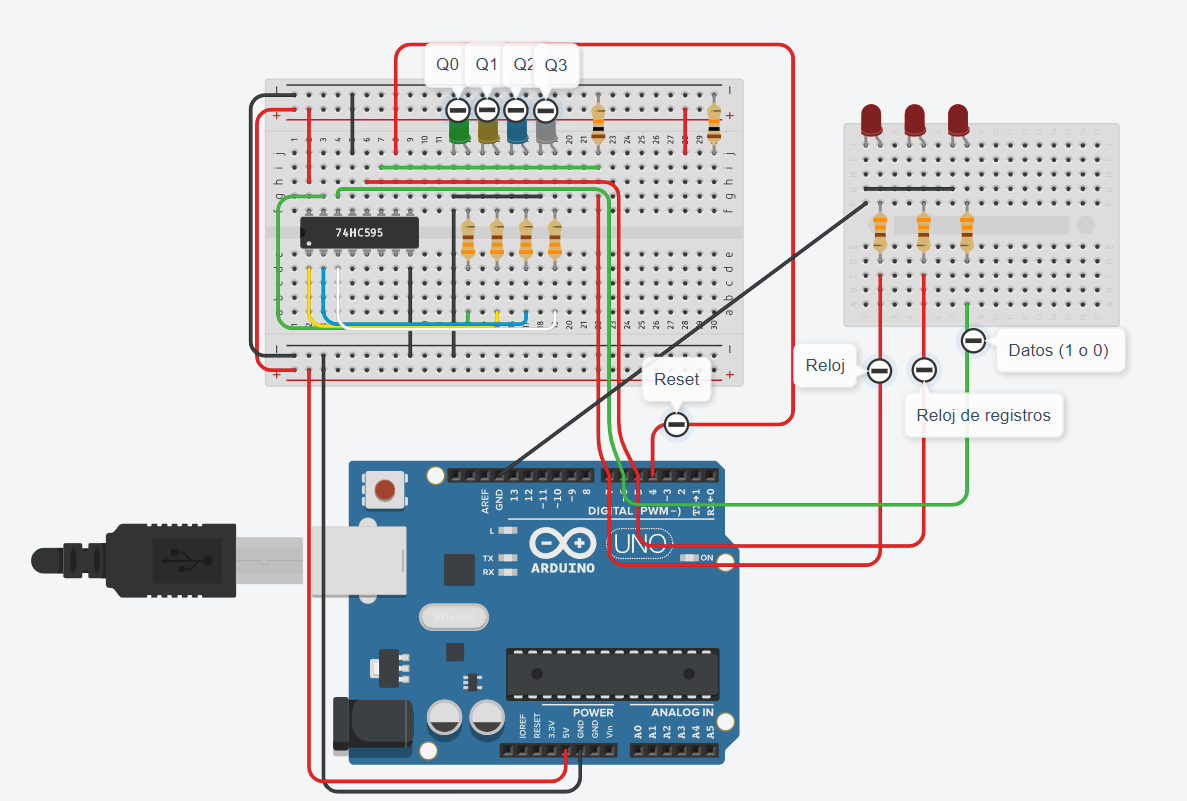
\includegraphics[width=7cm]{montaje1.PNG}
\centering
\caption{Montaje con 74HC595 y Arduino}
\end{figure}
\noindent
Código del Arduino con 74HC595:
\begin{lstlisting}[style=C++]
void setup()
{
  for(int i=4;i<8;i++){
  	pinMode(i, OUTPUT);
  }  
}
int binario[16]={0,0,0,1,0,1,1,0,0,1,1,0,1,0,0,0};
void loop()
{
  digitalWrite(4, LOW);
  digitalWrite(4, HIGH);
  digitalWrite(5, LOW);
  for(int i=0;i<16;i++){//debe recorrer todo el arreglo
    digitalWrite(5, LOW);
    if(binario[i]==1) digitalWrite(6, HIGH);
    else digitalWrite(6, LOW);
    delay(50);
    digitalWrite(7, HIGH);
    if((i+1)%4==0) digitalWrite(5, HIGH);//debe ser multiplo de la particion
    delay(450);
    digitalWrite(7, LOW);
    digitalWrite(5, LOW);
    digitalWrite(6, LOW);
    delay(500); 
  }
}
\end{lstlisting}
\vspace{2cm}
\subsubsection{Comunicación serial entre Arduinos}
Para enviar la información se usan dos pines digitales en cada Arduino, configurándolos como pines de entradas y salida para el receptor y transmisor respectivamente. Uno de los pines es para el reloj principal (pin 2 en el Arduino de la derecha)  y el otro para los datos en forma serial (pin 3 en el Arduino de la derecha). Los pulsos de reloj son generados internamente en el Arduino transmisor con ayuda de un ciclo y diferentes delay como se muestra en el código del Arduino 1 (TX-Izquierdo).
Se usa una variable global denominada tiempo que permite configurar el periodo de reloj y velocidad de transmisión de los datos.\\

En el Arduino receptor se usa un condicional que detecte si hay un flanco de subida en el reloj principal, y si lo hay se imprime en la consola serial 1 o 0 según el valor que haya en el pin de datos, ya sea un HIGH o un LOW. La impresión por consola es solo una medida de controlar el correcto funcionamiento del montaje, posteriormente los datos se usarán con otro objetivo como convertirlos a decimal.\\

Durante la implementación se presentó la dificultad de que el receptor tomaba varias veces el mismo valor debido a que la función loop se repite mucho más rápido de lo que cambian el reloj. Para solucionarlo, se redujo drásticamente el tiempo en alto del reloj hasta 0.5 ms, de forma que el receptor pueda recibir solo un dato a la vez y no varias veces el mismo dato generando errores. El montaje se muestra en la Figura 8.

\begin{figure}[!ht] 
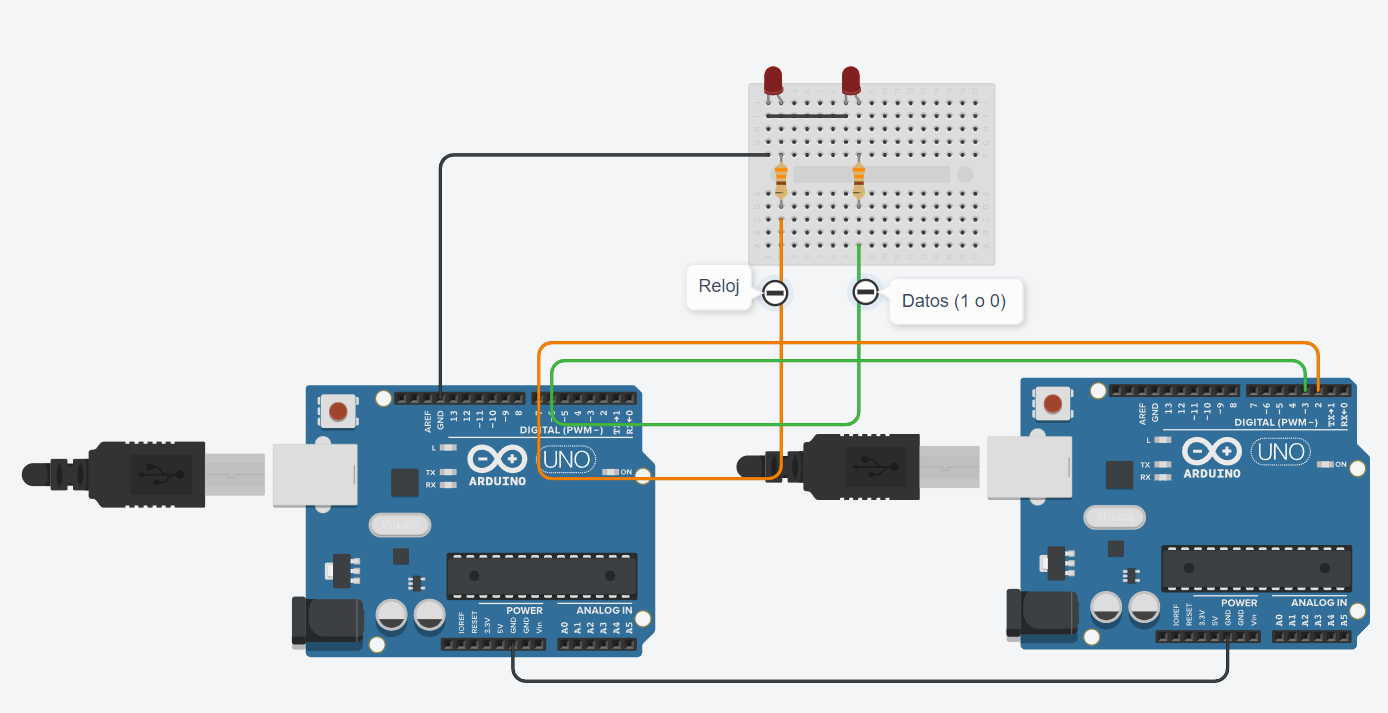
\includegraphics[width=7cm]{montajeSerial.PNG}
\centering
\caption{Montaje de Arduinos en comunicación serial}
\end{figure}

\noindent
Código del Arduino 1 (TX-Izquierdo):

\begin{lstlisting}[style=C++]
void setup()
{
  for(int i=4;i<8;i++){
  	pinMode(i, OUTPUT);
  }  
}
int binario[24]={0,1,0,1,1,1,1,1,0,1,0,0,0,1,0,1,0,1,1,1,1,1,1,1};
int tiempo=500;//variable tiempo que define el periodo del reloj
void loop()
{
  digitalWrite(4, LOW);
  digitalWrite(5, LOW);
  digitalWrite(4, HIGH);
  for(int i=0;i<24;i++){//debe recorrer todo el arreglo
    digitalWrite(5, LOW);
    if(binario[i]==1) digitalWrite(6, HIGH);
    else digitalWrite(6, LOW);
    delay(tiempo/20);//50
    digitalWrite(7, HIGH);
    if((i+1)%8==0) digitalWrite(5, HIGH);//debe ser multiplo de la particion
    delay(0.5); //un tiempo muy bajo de reloj, garantiza que solo se tome un dato en el otro Arduino
    digitalWrite(7, LOW);
    delay(tiempo-tiempo/2-tiempo/20-0.5);
    digitalWrite(5, LOW);
    digitalWrite(6, LOW);
    delay(tiempo/2); 
  }
}
\end{lstlisting}

\noindent
Código del Arduino 2 (RX-Derecho):

\begin{lstlisting}[style=C++]
void setup()
{
  for(int i=2;i<4;i++){
  	pinMode(i, INPUT);
  } 
  Serial.begin(9600);
}
bool dato=LOW,datoAnterior=LOW;
void loop()
{
  dato=digitalRead(2);
  if(dato==HIGH && datoAnterior==LOW){ //detector de flancos
  	if(digitalRead(3)==HIGH) Serial.println(1);
    else if(digitalRead(3)==LOW) Serial.println(0);
  }
  datoAnterior==dato;
  Serial.println(1);
}
\end{lstlisting}

\subsubsection{Módulo de desencriptación}
El módulo de desencriptación consiste en un circuito de lógica combinacional que compara los 8 bits que salen del 74HC595 con los 8 bits del número de referencia que en nuestro caso es el \textbf{127}.\\

Para comparar bit a bit se requieren 8 compuertas XOR, en una de las entradas entra el bit que sale del integrado, y en la otra entrada el bit correspondiente al número de referencia. Según la tabla de verdad de la compuerta XOR, mostrada en la Figura 9, cuando ambas entradas son iguales, la salida es cero, por tanto, se usan negadoras para que cuando esto ocurra se tenga un valor True en la salida, de esta forma se requieren 8 compuertas NOT. Las 8 salidas de las negadoras alimentan la entrada de un sistema de compuertas AND cuyo objetivo es comparar que todas las salidas de las NOT sean 1, es decir, que todos los bits sean iguales, por lo que se necesitan 7 compuertas AND.\\


\begin{figure}[!ht] 
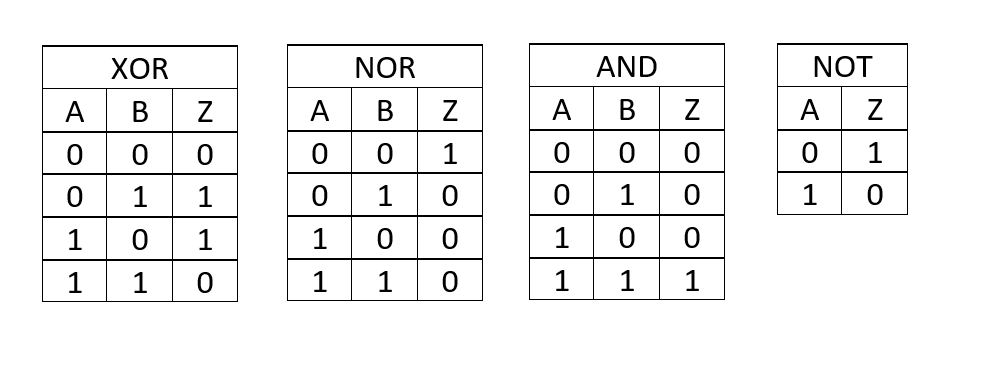
\includegraphics[width=10cm]{compuertas.png}
\centering
\caption{Tablas de verdad de las compuertas XOR, NOR, AND y NOT}
\end{figure}

Dentro del catálogo de integrados de compuertas lógicas disponibles en el aplicativo Tinkercad tenemos los siguientes:
\begin{itemize}
    \item 74HC21: dos compuertas AND de 4 entradas
    \item 74HC08: 4 compuertas AND de dos entradas
    \item 74HC86: 4 compuertas XOR de dos entradas
    \item 74HC02: 4 compuertas NOR de dos entradas
    \item 74HC04: 6 compuertas negadoras\\
\end{itemize}

De esta forma, y considerando integrados que solo dispongan de compuertas de dos entradas se necesitarían alrededor de 6 integrados en total para realizar el montaje planteado en la Figura 10.

\begin{figure}[!h] 
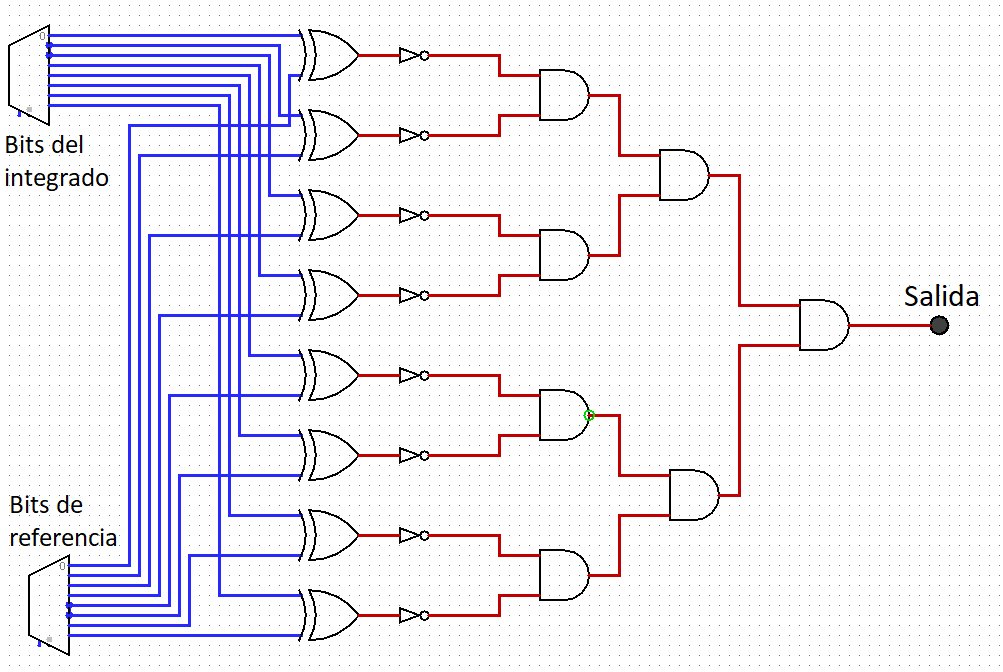
\includegraphics[width=8cm]{logica1.png}
\centering
\caption{Circuito de lógica combinacional propuesto}
\end{figure}

Analizando un poco mejor el circuito y usando álgebra de bool, se observa que la expresión correspondiente a las AND cuyas entradas son negadas, puede transformarse aplicando la ley de De Morgan así: $\bar{A}\bar{B} = \overline{A+B}$.

Con esto estamos sustituyendo la AND y las negadoras, por una sola compuerta NOR y reduciendo el número de integrados de 6 a 4. También se puede usar una compuerta AND de 4 entradas para reemplazar las 3 AND de 2 entradas en la parte final del circuito. Aunque esto no reduce los integrados a usar, sí facilita la conexión de los chips durante el montaje. Esta simplificación se muestra en la Figura 11.\\

\begin{figure}[!ht] 
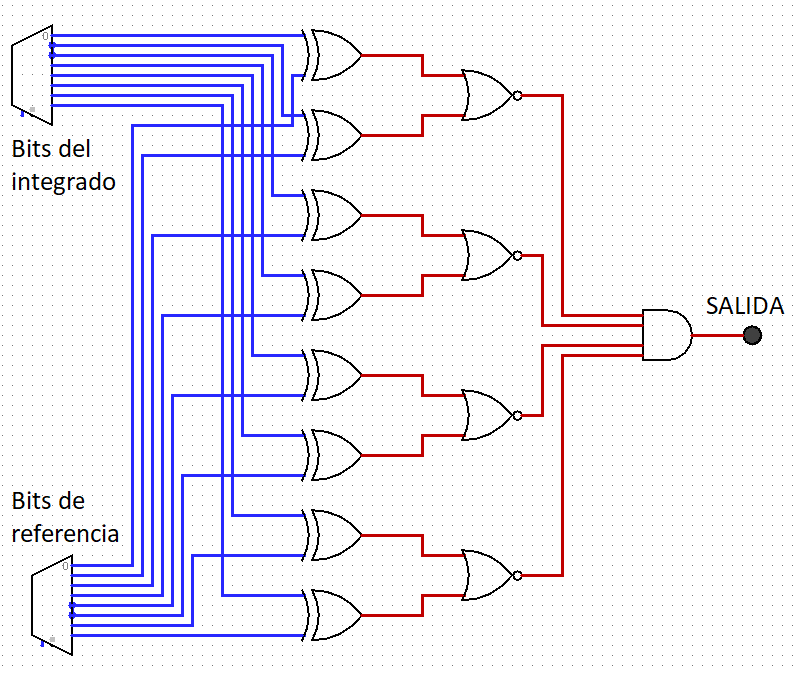
\includegraphics[width=8cm]{logica2.png}
\centering
\caption{Circuito de lógica combinacional simplificado}
\end{figure}

Con el esquema planteado, se monta el circuito en Tinkercad, usando una fuente de alimentación de 5 V, DIP conmutadores para simular las entradas, los integrados de compuertas lógicas \textbf{74HC86 (XOR)}, \textbf{74HC02 (NOR)}, \textbf{74HC21 (AND)} y un diodo LED que se enciende cuando ambos números son iguales.\\

\begin{figure}[!ht] 
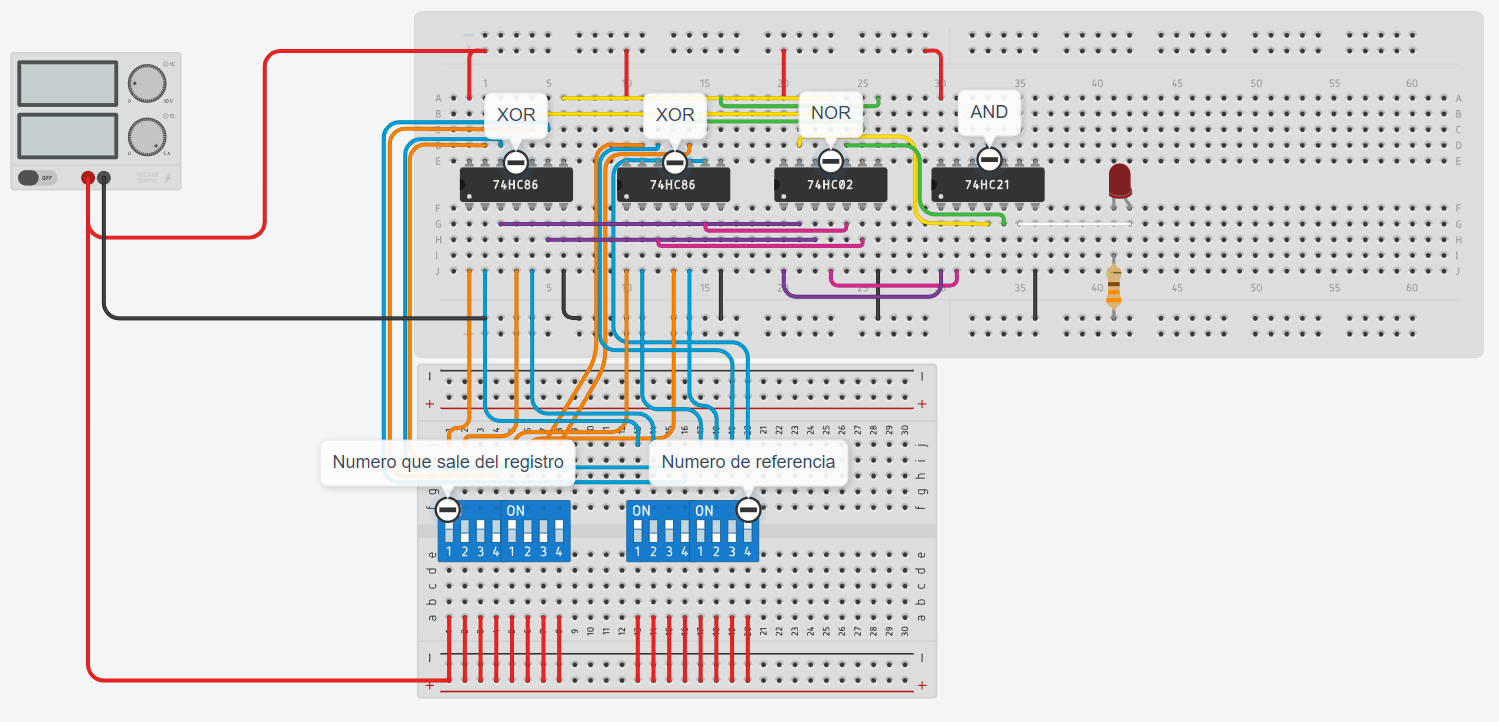
\includegraphics[width=10cm]{montajeCompuertas.PNG}
\centering
\caption{Implementación del circuito de lógica combinacional simplificado}
\end{figure}

Para la construcción final, el DIP conmutador "Número que sale del registro" será reemplazado por las 8 salidas del 74HC595 (Registro de desplazamiento), mientras que el otro DIP conmutador no cambiará, y siempre tendrá el número de referencia 127, o cualquier otro pedido durante su ejecución.
\vspace{4cm}
\subsubsection{Codigos del Arduino tansmisor y Arduino receptor}
Debido a que en el problema, se entrega un arreglo de enteros es necesario elaborar un programa que realice la conversión de decimal a binario en el transmisor y otro que realice la conversion binario a decimal para luego aplicar las reglas de desencriptacion en el receptor. Inicialmente, la implementación se realiza en QT, para apoyarse del depurador y realizar pruebas. Posteriormente, se lleva el código a ambos Arduinos. El código se encuentra a continuación:

\noindent


\begin{lstlisting}[style=C++]
#include <iostream>
using namespace std;

int main()
{
//CODIGO DEL TRANSMISOR
int tam=19, n, num[19]={50,127,13,240,49,89,17,127,170,93,27,127,1,2,3,127,1,1,3};
int *bin = new int[8*tam];
for (int i=0,test=1;i<tam;i++, test++) {
    n=num[i];
    for (int j=7,k=8*test-1;j>-1;j--) {
        if (n%2==0) {
            bin[k]=0; //se empieza a llenar desde la posicion final de la particion de 8 bits
        }
        else{
            bin[k]=1;
        }
        n/=2;
        k--;
    }
}
for (int i=0;i<tam*8;i++) {//Imprime el arreglo (CONTROL)
    cout<<*(bin+i);
    if((i+1)%8==0) cout<<"|";//Separador de bits
}
cout<<endl;

//CODIGO DEL RECEPTOR
//En el Arduino se debe inicializar un arreglo de la misma longitud tam que se ira llenando de
//los enteros ya convertidos

int num_recuperado[19]={0}, potencia=128, test, count=0, sum=0,mean=0; //n
n=0;
bool flag=false;

for (int i=0,j=0;i<tam*8;i++) { //Este ciclo recorre el arreglo binario, simulando la entrada de los datos via serial (se quita en tinkercad)
    test=bin[i]; //control
    n +=bin[i]*potencia;//Los bits entran desde el mas hasta el menos significativo,
    potencia/=2;        //por lo que se multitplican por un numero multiplo de 2 (de acuerdo al numero total de bits, 2^7)
                        //que se dividide en cada iteracion

    if ((i+1)%8==0) { //Cada 8 bits se verifica si el numero convertido es la bandera
        if (flag == true) {
            sum+=n; //Se suman los datos
            //num_recuperado[j]=n;
            //j++;
            count++;
            if (count == 3) {
                //Para calcular la media y redondear
                if (10*(sum%3)/3 >= 5) {
                    mean = sum/3+1;
                }
                else {
                    mean = sum/3;
                }
                num_recuperado[j]=mean;
                j++;
                mean=0;
                sum=0;
                count=0;
                flag = false;
            }
        }
        if(n==127){ //Esto simula la salida del circuito de logica combinacional
            flag = true; //Activa una bandera booleana que estara activa 3 bytes
        }
        //Se reinician las variables y se aumenta el contador
        n=0;
        potencia=128;

    }

}
for (int i=0;i<tam;i++) {//Imprime el arreglo (CONTROL)
    cout<<num_recuperado[i];
    cout<<"|";//Separador de bits
}
cout<<endl;

delete[] bin;
return 0;
}

\end{lstlisting}

La primera parte del código consiste en un for que recorre el arreglo de enteros, y a cada elemento le realiza la división sucesiva por dos para obtener la conversión a binario. El arreglo de bits se llena de forma tal que el bit más significativo quede a la derecha de cada partición de 8 bits.
Luego se imprime el arreglo para comprobar que el arreglo de bits está correcto.\\

La segunda parte, convierte el arreglo de bits simulando la entrada serial del Arduino receptor con ayuda de un for, a medida que se convierten los números se comparan con una sentencia if, que simula la salida del circuito de lógica combinacional, y activa una bandera que permite realizar el promedio con redondeo de los 3 siguientes datos al valor de referencia, que en nuestro caso es 127.

\subsubsection{Ensamble de los módulos anteriores}
Una vez garantizado el correcto funcionamiento de cada módulo por separado y teniendo los códigos para la transmisión y recepción, se procede a ensamblarlos y realizar las conexiones respectivas. Primero se reemplaza el DIP conmutador que simula la salida de los datos del integrado en el módulo de encriptación, por las salidas reales del 74HC595 y se conecta la salida del circuito de lógica combinacional a pin 4 del Arduino receptor. Luego se conectan ambos Arduinos y se cargan los códigos para permitir la comunicación serial. Se opta por conservar algunos montajes de LED como elementos de control. El montaje se puede apreciar en la Figura 13.\\

Al llevar los códigos a los Arduinos se deben hacer algunas modificaciones como reemplazar las salidas de consola por la respectiva sintaxis de salida por la consola serial, definir variables extra para iterar los arreglos y definir el arreglo que se llevara al LCD para desplegar la información. Estos códigos y los anteriormente mencionados en todo el documento se pueden encontrar en la carpeta Arduino del repositorio compartido.\\

Durante la ejecución de las pruebas se notó un problema de sincronización con el Arduino receptor, este se debía a que la inicializacion de las librerias que permiten desplegar mensajes en el LCD tardaba mas de lo esperado, y por tanto el receptor comenzaba a procesar los datos a partir del segundo bit de todo el arreglo. Esto se solucionó agregando un pequeño delay en el transmisor de forma que le de tiempo al receptor de estar listo antes de comenzar a enviar la informacion en forma serial.\\

\begin{figure}[!ht] 
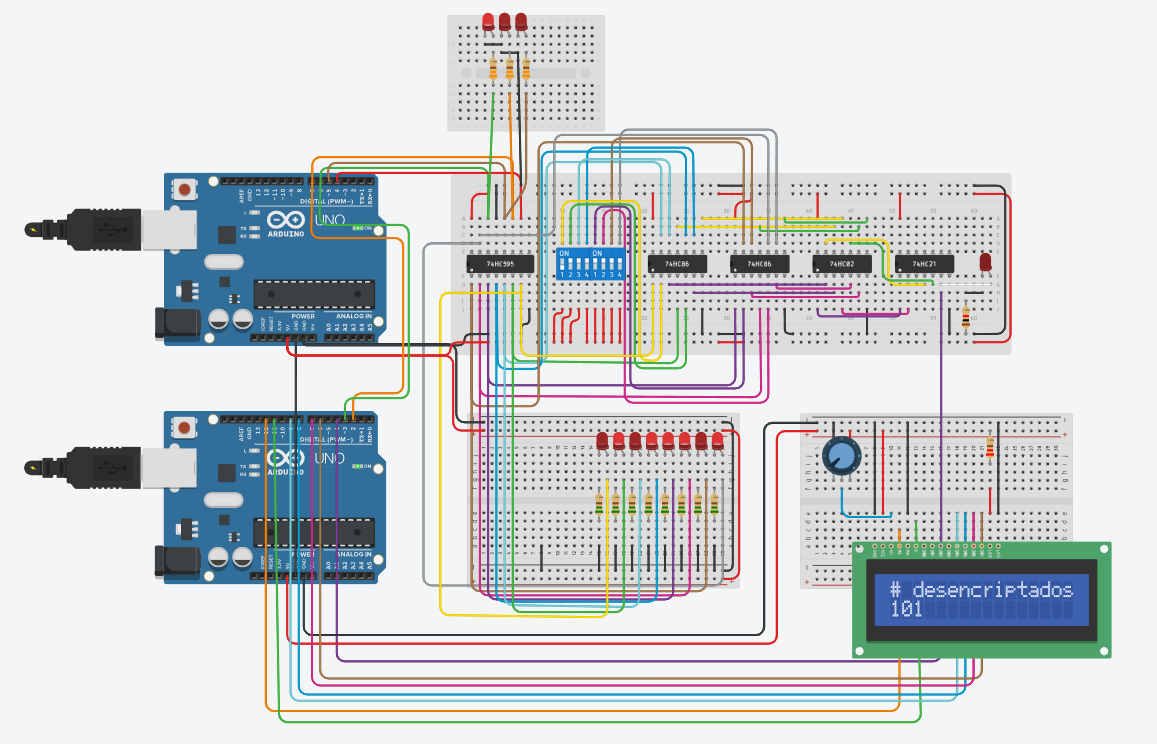
\includegraphics[width=12cm]{esquemaEnsamble.PNG}
\centering
\caption{Ensamble de los módulos anteriores}
\end{figure}
\vspace{2cm}
\noindent
Código del Arduino 1 (TX-Superior):

\begin{lstlisting}[style=C++]
int tam=19, n, num[19]={50,127,13,240,49,89,17,127,170,93,27,127,1,2,3,127,1,1,7};
int *bin = new int[8*tam];
int tiempo=50;//variable tiempo que define el periodo del reloj


void setup()
{
  for(int i=4;i<8;i++){
  	pinMode(i, OUTPUT);
  }  
  
  for (int i=0,test=1;i<tam;i++, test++) {
    n=num[i];
    for (int j=7,k=8*test-1;j>-1;j--) {
      if (n%2==0) {
        bin[k]=0; //se empieza a llenar desde la posicion final de la particion de 8 bits
      }
      else{
        bin[k]=1;
      }
      n/=2;
      k--;
    }
  }
  delay(100); //Delay que corrige el atraso generado por la inicializacion del LCD
}

void loop()
{
  digitalWrite(4, LOW);
  digitalWrite(5, LOW);
  digitalWrite(4, HIGH);
  
  
  for(int i=0;i<8*tam;i++){//debe recorrer todo el arreglo
    digitalWrite(5, LOW);
    if(bin[i]==1) digitalWrite(6, HIGH);
    else digitalWrite(6, LOW);
    delay(tiempo/20);//50
    digitalWrite(7, HIGH);
    if((i+1)%8==0) digitalWrite(5, HIGH);//debe ser multiplo de la particion
    
    delay(0.5); //un tiempo muy bajo de reloj, garantiza que solo se tome un dato en el otro arduino
    digitalWrite(7, LOW);
    delay(tiempo-tiempo/2-tiempo/20-0.5);
    digitalWrite(5, LOW);
    digitalWrite(6, LOW);
    delay(tiempo/2); 
    
    
  }
  
  delete[] bin;
}
\end{lstlisting}

\noindent
Código del Arduino 2 (RX-Inferior):

\begin{lstlisting}[style=C++]
#include <LiquidCrystal.h>
const int rs = 12, en = 11, d4 = 9, d5 = 8, d6 = 7, d7 = 6;
LiquidCrystal lcd(rs, en, d4, d5, d6, d7);

int tam=19,num_recuperado[19]={0},potencia=128,count=0,sum=0,mean=0,n=0,bin;
int i=0,j=0,k=0,nFlag=0;
bool flag=false;
bool dato=LOW,datoAnterior=LOW;

void setup()
{
  for(int i=2;i<=4;i++){
  	pinMode(i, INPUT);
  } 
  Serial.begin(9600);
  // Se inicia el LCD con el numero de columnas y filas:
  lcd.begin(16, 2);
}


void loop()
{
  dato=digitalRead(2);
  if(dato==HIGH && datoAnterior==LOW){ //detector de flancos
    
    //Serial.println("reloj");
    if(digitalRead(3)==HIGH){
      Serial.print(1);
      bin=1;
    }
    else if(digitalRead(3)==LOW){
      Serial.print(0);
      bin=0;
    }
    
    n +=bin*potencia;//Los bits entran desde el mas hasta el menos significativo,
    potencia/=2;
    
    if ((i+1)%8==0) { //Cada 8 bits se verifica si el numero convertido es la bandera
        if (flag == true) {
          sum+=n; //Se suman los datos
          count++;
          if (count == 3) {

            //Para calcular la media y redondear
            if (10*(sum%3)/3 >= 5) {
              mean = sum/3+1;
            }
            else {
              mean = sum/3;
            }
            Serial.println(" ");
			Serial.print("Media= "); Serial.print(mean);
            num_recuperado[j]=mean;
            j++;
            mean=0;
            sum=0;
            count=0;
            flag = false;
            
          }
        }

          if(digitalRead(4)==HIGH){ //Bandera de la logica combinacional
            flag = true; //Activa una bandera booleana que estara activa 3 bytes
            nFlag++; //variable que cuenta el numero de banderas true

          }

        //Se reinician las variables y se aumenta el contador
        n=0;
        potencia=128;
      	Serial.println(" ");

      }
  i++;
  }
  
  
  if(i>=tam*8){
    
    int *arreglo_final = new int[nFlag];//Este sera el arreglo final
    
    for (int j=0;j<nFlag;j++) {//Imprime el arreglo (CONTROL)
      arreglo_final[j]=num_recuperado[j];
      Serial.print(arreglo_final[j]);
      Serial.print(",");//Separador de bits
    }
    
    
    //Codigo del LCD
    // Se enciende el scroll automatico
    //lcd.autoscroll();

    // se posiciona el cursor en (0,0):
    lcd.setCursor(0, 0);

    // Imprme un mensaje en el LCD.
    lcd.print("# desencriptados");

    // se posiciona el cursor en (0,1):
    lcd.setCursor(0, 1);

    // imprime los elementos de la lista separados con espacio:
    
    lcd.print(arreglo_final[k]);
    lcd.print(' ');
    delay(500);
    k++;
    if(k==nFlag){
    	k=0;
    }
    
    // Se apaga el scroll automatico
    //lcd.noAutoscroll();

    // Se limpia el lcd para el siguiente ciclo
    //lcd.clear();
    
    //i=0;
    Serial.println(" ");
    delete[] arreglo_final;
  }
  datoAnterior==dato;
}

\end{lstlisting}

\subsubsection{Ejemplo de funcionamiento}
A continuación se muestra la salida en el Arduino receptor, cuando el arreglo de números es\\
50,127,13,240,49,89,17,127,170,93,27,127,1,2,3,127,1,1,7. 
Se espera que el el arreglo final tenga 4 números, pues el arreglo inicial contiene 4 banderas.\\
Puede verse en la Figura 14 que los resultados son como se esperaban y que el arreglo final es 101,97,2,3. Después de acá el receptor no toma mas datos, sino que se queda imprimiendo los valores uno a uno en el LCD.

\begin{figure}[!ht] 
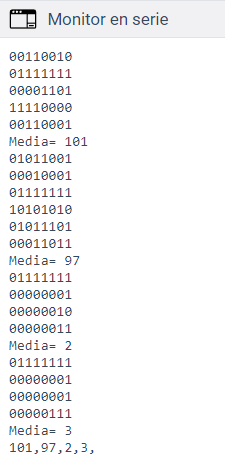
\includegraphics[width=4cm]{ejemploFuncionamiento.PNG}
\centering
\caption{Ejemplo de funcionamiento del circuito completo}
\end{figure}

\vspace{6cm}
\section{Conclusiones} \label{conclusiones}
\begin{itemize}
    \item Las investigaciones del funcionamiento del circuito integrado 74HC595 que permite paralelizar los datos así como la de otros conceptos básicos fueron cruciales para darle solución al problema planteado, de esta forma siempre que se vaya a desarrollar una solución para cualquier tipo de problema, es fundamental adquirir los conocimientos previos necesarios para llevarla a cabo. 
    \item La construcción modular de sistemas es generalmente la estrategia mas adecuada para afrontar un problema, pues permite enfocarse en la implementación de cada parte con mayor atención, además de facilitar la solución y detección de errores.
    \item El uso de herramientas como TinkerCAD y QT Creator facilitan el desarrollo de la solucion de problemas, pues mientras la primera simula de manera muy exacta la implementacion de circuitos y nos permite hacer montajes cercanos a la realidad, la segunda ofrece ayudas como la correccion de sintaxis y el uso del depurador, permitiendo centrarse mas en la esencia logica de la programacion que en la correccion de escritura. Ademas de la interoperabilidad entre ambas herramientas pues las dos se trabajan con lenguaje C++. 
\end{itemize}
\vspace{5cm}
\bibliographystyle{IEEEtran}
\bibliography{references}

\end{document}
